\documentclass[10pt,aps,prb,twocolumn,amsmath,amssymb,floatfix]{revtex4-2}
\usepackage[dvipsnames]{xcolor}
\usepackage[colorlinks,allcolors=blue,plainpages=false,pdfpagelabels]{hyperref}
\usepackage{amsmath,bm}
\usepackage{tikz}
\usetikzlibrary{positioning, shapes}
\pgfdeclarelayer{background}
\pgfdeclarelayer{foreground}
\pgfsetlayers{background,main,foreground}
\usetikzlibrary{shapes.misc}
\tikzset{cross/.style={cross out, draw=black, minimum size=2*(#1-\pgflinewidth), inner sep=0pt, outer sep=0pt},cross/.default={1pt}}

\begin{document}

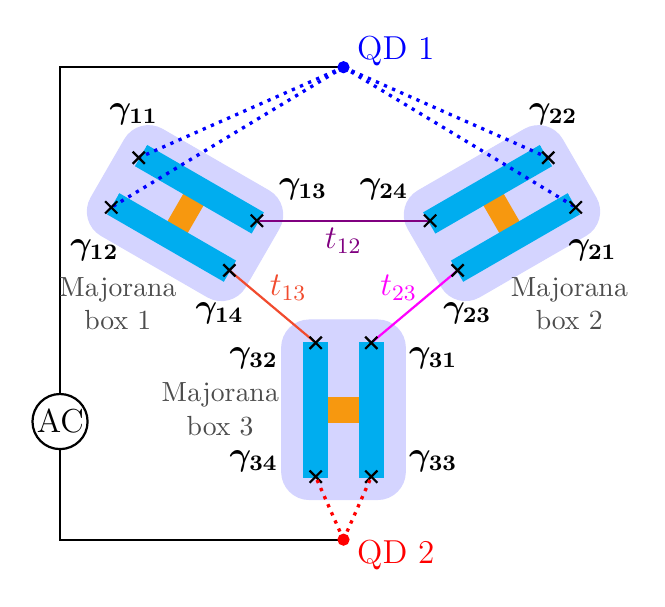
\begin{tikzpicture}[every text node part/.style={align=center}]

    \begin{pgfonlayer}{foreground}
    \filldraw [blue] (2.5, 1.0) circle (2pt) node[blue, anchor=west] at (2.55, 1.2) {\large QD $1$};

    \draw[dotted, blue, very thick] (2.5, 1.0) -- (-0.1, -0.15) 
    ;
    \draw[dotted, blue, very thick] (2.5, 1.0) -- (-0.45, -0.78) 
    ;

    \draw[dotted, blue, very thick] (2.5, 1.0) -- (4.1 +1, -0.15) 
    ;
    \draw[dotted, blue, very thick] (2.5, 1.0) -- (4.45 +1, -0.78) 
    ;

    \draw[black, thick] (-0.1, -0.15) node[cross=3pt, rotate=90]{} node[anchor=west] at (-0.6, 0.1 + 0.3) {\large $\bm{\gamma_{11}}$};
    \draw[black, thick] (1.4, -0.95) node[cross=3pt, rotate=90]{} node[anchor=west] at (1.0 +0.55, -0.7 + 0.15) {\large $\bm{\gamma_{13}}$};
    \draw[black, thick] (-0.45, -0.78) node[cross=3pt, rotate=90]{} node[anchor=west] at (-0.95-0.15, -0.53-0.8){\large $\bm{\gamma_{12}}$};
    \draw[black, thick] (1.05, -1.58) node[cross=3pt, rotate=90]{} node[anchor=west] at (0.64 -0.15, -1.33-0.8) {\large $\bm{\gamma_{14}}$};

    \draw[black, thick] (4.1 +1, -0.15) node[cross=3pt, rotate=90]{} node[anchor=east] at (4.6 +1, 0.1+0.3) {\large $\bm{\gamma_{22}}$};
    \draw[black, thick] (2.6 +1, -0.95) node[cross=3pt, rotate=90]{} node[anchor=east] at (3.0 +1 -0.55, -0.7+0.15){\large $\bm{\gamma_{24}}$};
    \draw[black, thick] (4.45 +1, -0.78) node[cross=3pt, rotate=90]{} node[anchor=east] at (4.95 +1 + 0.15, -0.53 -0.8){\large $\bm{\gamma_{21}}$};
    \draw[black, thick] (2.95 +1, -1.58) node[cross=3pt, rotate=90]{} node[anchor=east] at (3.36 +1 +0.15, -1.33 -0.8){\large $\bm{\gamma_{23}}$};

    \filldraw [red] (2.5, -5.0) circle (2pt) node[red, anchor=west] at (2.55, -5.2) {\large QD $2$};
    \filldraw [color=black, fill=white, thick] (-1.1, -3.5) circle (0.35) node[anchor=west] at (0.575-2.1, -3.5) {\large AC};
    \draw[dotted, red, very thick] (2.5, -5.0) -- (2.5-0.212-0.142, -2.5 -1.70) 
    ;
    \draw[dotted, red, very thick] (2.5, -5.0) -- (2.5+0.212 +0.142, -2.5 -1.70) 
    ;
    \end{pgfonlayer}

    %Link tunnels between Majorana boxes%
    \draw[violet, thick] (1.4, -0.95) -- (2.6 +1, -0.95) node[violet] at (2.5, -1.2) {\large $t_{12}$};
    \draw[Magenta, thick] (2.95 +1, -1.58) -- (2.5 + 0.212 + 0.141, -2.5) node[Magenta] at (3.4015 - 0.2, -1.8) {\large $t_{23}$};
    \draw[RedOrange, thick] (2.05 -1, -1.58) -- (2.5 - 0.212 - 0.141, -2.5) node[RedOrange] at (5 -3.4015 + 0.2, -1.8) {\large $t_{13}$};

    %Driving tunnel between QDs%
    \draw[black, thick] (2.5, 1.0) -- (-1.1, 1.0) -- (-1.1, -5.0) -- (2.5, -5.0);
    
    \begin{scope}[rotate around= {15 : (0, 0)}]
    \begin{pgfonlayer} {background}
    \filldraw[blue!17, rounded corners=10pt] (0, 0.4)  -- (1.6, -1.2) -- (0.5, -2.3) -- (-1.1, -0.7) -- cycle ;
    \begin{pgfonlayer} {background}
        \filldraw[YellowOrange, thick] (0.3, -0.7) -- (0.5, -0.9) -- (0.2, -1.2) -- (0, -1);
    \end{pgfonlayer}
    \end{pgfonlayer}
    \filldraw[cyan, thick] (0, 0) -- (1.2, -1.2) -- (1.0, -1.4) -- (-0.2, -0.2);
    \filldraw[cyan, thick] (-0.5, -0.5) -- (0.7, -1.7) -- (0.5, -1.9) -- (-0.7, -0.7);
    \end{scope}

    \begin{scope}[rotate around= {-15 : (4 +1, 0) }]
    \begin{pgfonlayer} {background}
        \filldraw[blue!17, rounded corners=10pt] (4 +1, 0.4) -- (2.4 +1, -1.2) -- (3.5 +1, -2.3) -- (5.1 +1, -0.7)  --cycle ;
    \begin{pgfonlayer}{background}
        \filldraw[YellowOrange, thick] (4.7, -0.7) -- (4.5, -0.9) -- (4.8, -1.2) -- (5, -1);
    \end{pgfonlayer}
    \end{pgfonlayer}
    \filldraw[cyan, thick] (4 +1, 0) -- (2.8 +1, -1.2) -- (3.0 +1, -1.4) -- (4.2 +1, -0.2);
    \filldraw[cyan, thick] (4.5 +1, -0.5) -- (3.3 +1, -1.7) -- (3.5 +1, -1.9) -- (4.7 +1, -0.7);
    \end{scope}

    \begin{pgfonlayer} {background}
        \filldraw[blue!17, rounded corners=10pt] (2.5-0.212-0.283 - 0.29, -2.5 + 0.29) rectangle (2.5+0.212+0.283 + 0.29, -2.5 -1.70 - 0.29) ;
        \begin{pgfonlayer}{background}
            \filldraw[YellowOrange, thick] (2.288, -2.5 - 0.7) rectangle (2.712, -4.2 + 0.7);
        \end{pgfonlayer}
    \end{pgfonlayer}
    \filldraw[cyan, thick] (2.5-0.212, -2.5)  rectangle (2.5-0.212-0.283, -2.5 -1.70);
    \filldraw[cyan, thick] (2.5+0.212, -2.5)  rectangle (2.5+0.212+0.283, -2.5 -1.70);

    \draw[black, thick] (2.5-0.212-0.141, -2.5) node[cross=3pt, rotate=90]{} node[anchor=east] at (2.5-0.212-0.141 -0.35, -2.5-0.2) {\large $\bm{\gamma_{32}}$};
    \draw[black, thick] (2.5-0.212-0.141, -2.5-1.70) node[cross=3pt, rotate=90]{} node[anchor=east] at (2.5-0.212-0.141 -0.35, -2.5-1.70 + 0.2){\large $\bm{\gamma_{34}}$};
    \draw[black, thick] (2.5 + 0.212 + 0.141, -2.5) node[cross=3pt, rotate=90]{} node[anchor=west] at (2.5+0.212+0.141 +0.35, -2.5-0.2) {\large $\bm{\gamma_{31}}$};
    \draw[black, thick] (2.5+0.212+0.141, -2.5-1.70) node[cross=3pt, rotate=90]{} node[anchor=west] at (2.5+0.212+0.141 +0.35, -2.5-1.70 + 0.2){\large $\bm{\gamma_{33}}$};

    \draw[black!70] node[anchor=east] at (0.5, -2.3 +0.3) { Majorana \\ box $1$};
    \draw[black!70] node[anchor=west] at (4.5, -2.3 +0.3) { Majorana \\ box $2$};
    \draw[black!70] node[anchor=east] at (1.8, -2.79 -0.55) { Majorana \\ box $3$};
      
\end{tikzpicture}

\end{document}